
{As discussed above there are 3 cases/methods to find the density of the metal block as there are 3 ways to find the volume of the metal block and there is only one way to find the mass of the metal block.}

\section{{Experiment 1}}

	\subsection{{Standard Deviation of Uncertainity}}

		{}
		
			$$s = \sqrt{\frac{1}{n - 1}\sum_{i = 1}^{n}{\left(x_{i} - \bar{x}\right)}^2}$$
			
			$$s^2 = \frac{\sum{\left(x_{i} - \bar{x}\right)}^2}{n - 1} \approx 0.08328$$

	\subsection{{Predicted Acceleration using $g\sin\theta$}}

		{}
		
			$$\left|\overrightarrow{a}\right| = g\sin\theta$$

			$$\left|\overrightarrow{a}\right| = 9.81\sin\left(15^{\circ} \pm 0.03^{\circ}\right) \approx 2.5 m/s^2 \pm 0.03 m/s^2$$

	\subsection{{Uncertainity}}

	{We have,}

		$$\Delta \overrightarrow{a} = 0.03 \times \frac{\pi}{180} \approx 5.3\times 10^{-4} m/s^2$$

\begin{figure}[H]
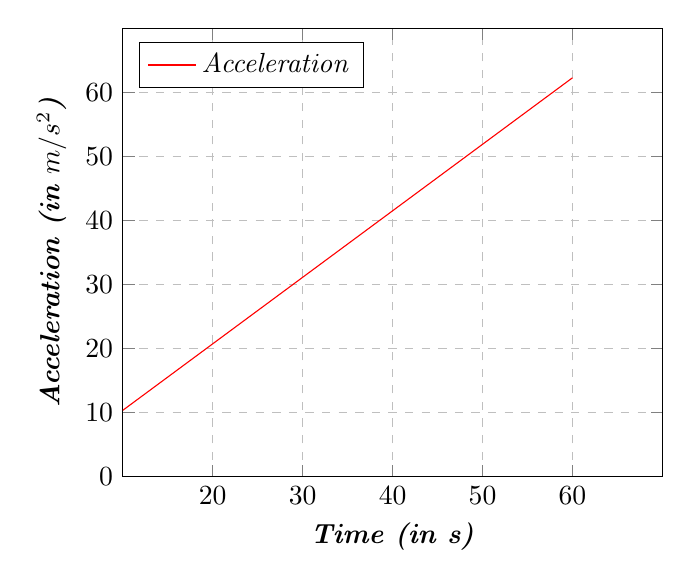
\begin{tikzpicture}
            \begin{axis}[
%                title={\textit{Graph in relation to the \textbf{experimental} \& \textbf{simulation} values of \textbf{drag force} versus \textbf{temperature}}},
                xlabel={\textbf{\textit{Time (in s)}}},
                ylabel={\textbf{\textit{Acceleration (in $m/s^2$)}}},
                xmin=10, xmax=70,
                ymin=0, ymax=70,
                xtick={20,30,40,50,60},
                ytick={0,10,20,30,40,50,60},
                legend pos=north west,
                ymajorgrids=true,
                xmajorgrids=true,
                grid style=dashed,
                legend entries={\textit{Acceleration}}
            ]

%			Methanol
            
			\addplot [
    	domain=0:60, 
    	samples=1000, 
    	color=red,
			]
	{(1.0385)*x + (-0.0473075)};
               
            \end{axis}
%            \caption{\textit{Graph in relation to the \textbf{experimental} \& \textbf{simulation} values of \textbf{drag force} versus \textbf{temperature}}}
        \end{tikzpicture}
        \caption{\textit{Graph in relation to the \textbf{regression line} of \textbf{acceleration} versus \textbf{time}}}}
		\end{figure}

%{Therfore we have,}

{}

\section{{Experiment 2}}

	\subsection{{Experimental Measurement of Acceleration}}

		$$\left|\overrightarrow{a}\right| = 1.7 m/s^2$$

		\begin{table}[H]
                \centering
                \begin{tabular}{|c|c|}
                \hline
                \hline
                {Components} & {Constants} \\
                \hline
                \hline
                \textit{x} component & $x = -3.323$ \\
                 & $b = -0.003531$ \\
                \hline
                \textit{y} component & $a = -4.723$ \\
                	& $b = 6.321$ \\                
				& $c = -0.0265$ \\ 
                \hline
                \hline
                \end{tabular}
                %\caption{}
                \label{}
    \end{table}

\begin{figure}[H]
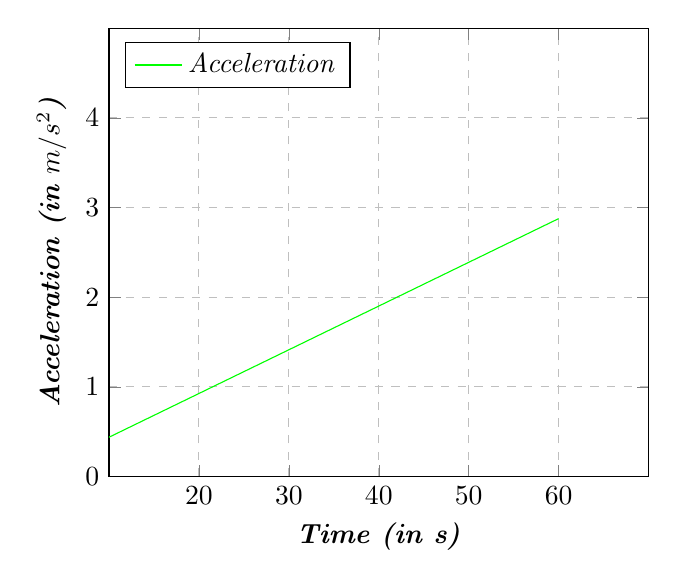
\begin{tikzpicture}
            \begin{axis}[
%                title={\textit{Graph in relation to the \textbf{experimental} \& \textbf{simulation} values of \textbf{drag force} versus \textbf{temperature}}},
                xlabel={\textbf{\textit{Time (in s)}}},
                ylabel={\textbf{\textit{Acceleration (in $m/s^2$)}}},
                xmin=10, xmax=70,
                ymin=0, ymax=5,
                xtick={20,30,40,50,60},
                ytick={0,1,2,3,4},
                legend pos=north west,
                ymajorgrids=true,
                xmajorgrids=true,
                grid style=dashed,
                legend entries={\textit{Acceleration}}
            ]

%			Ethanol

			\addplot [
    	domain=0:60, 
    	samples=1000, 
    	color=green,
			]
	{(0.04877)*x + (-0.04947)};
               
            \end{axis}
%            \caption{\textit{Graph in relation to the \textbf{experimental} \& \textbf{simulation} values of \textbf{drag force} versus \textbf{temperature}}}
        \end{tikzpicture}
        \caption{\textit{Graph in relation to the \textbf{regression line} of \textbf{acceleration} versus \textbf{time}}}}
		\end{figure}

\section{{Experiment 3}}

	\subsection{{Ball's Acceleration while in the air}}

		{We can calculate the acceleration by using the kinematic formula using the initial velocity, final velocity and time taken between the two intervals of the recorded velocities.}

			$$v_{f} = v_{i} + at$$
			
			$$a = \frac{v_{f} - v{i}}{t}$$
			
			$$\implies a = 2.36 m/s^2$$

\begin{figure}[H]
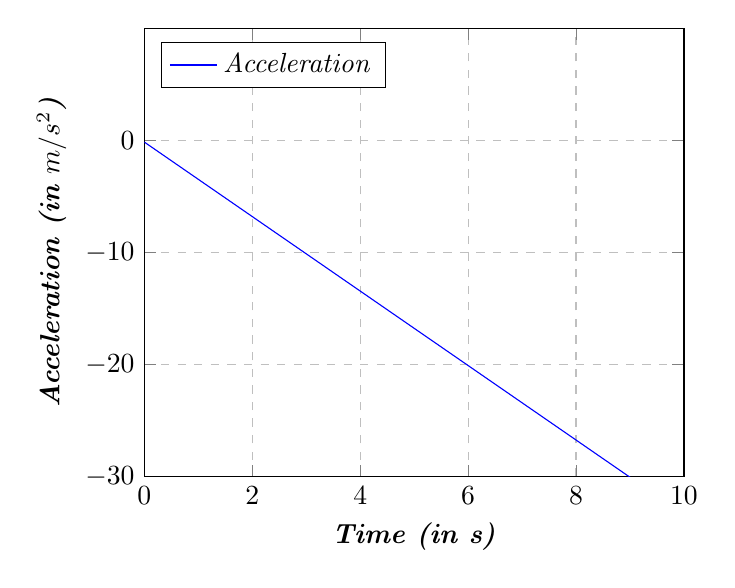
\begin{tikzpicture}
            \begin{axis}[
%                title={\textit{Graph in relation to the \textbf{experimental} \& \textbf{simulation} values of \textbf{drag force} versus \textbf{temperature}}},
                xlabel={\textbf{\textit{Time (in s)}}},
                ylabel={\textbf{\textit{Acceleration (in $m/s^2$)}}},
                xmin=0, xmax=10,
                ymin=-30, ymax=10,
                xtick={0,2,4,6,8,10},
                ytick={-30,-20,-10,0},
                legend pos=north west,
                ymajorgrids=true,
                xmajorgrids=true,
                grid style=dashed,
                legend entries={\textit{Acceleration}}
            ]

%			Propanol

			\addplot [
    	domain=0:10, 
    	samples=1000, 
    	color=blue,
			]
	{(-3.323)*x + (-0.1572)};

            \end{axis}
%            \caption{\textit{Graph in relation to the \textbf{experimental} \& \textbf{simulation} values of \textbf{drag force} versus \textbf{temperature}}}
        \end{tikzpicture}
        \caption{\textit{Graph in relation to the \textbf{regression line} of \textbf{acceleration} versus \textbf{time}}}}
		\end{figure}


